\documentclass{article}
\usepackage{mathtools}
\usepackage{color}
\usepackage[utf8]{inputenc}
\usepackage{mathtools}
\usepackage{graphicx}
\usepackage{placeins}
\begin{document}
\title{TDT4136 - Assignment 6}
\author{Filip F Egge}
\date{November 14, 2014}
\maketitle

\newpage
\section*{Planning - Question 1}
\subsection*{1. Figure with the planning graph and the highlighted plan}
	\FloatBarrier
	\begin{figure}[!htb]
		\caption{Graph}
		\centering
		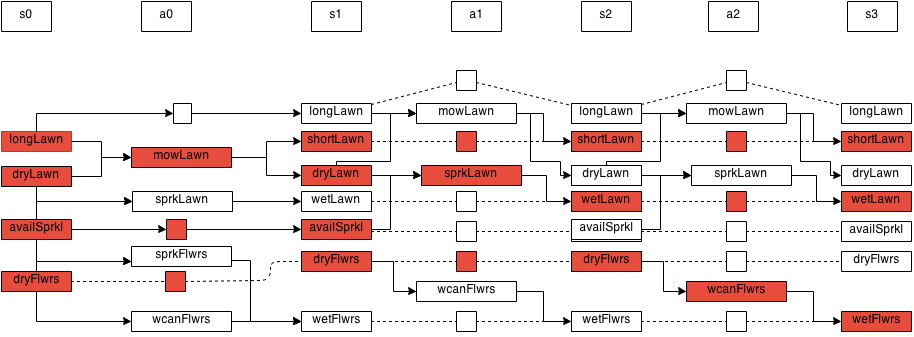
\includegraphics[width=0.9\textwidth]{graph.png}
	\end{figure}
\FloatBarrier
\subsection*{2. Explanation for why do you need (or not) to expand at each level}
	\subsubsection*{Level $S_0$}
		This is the initial state condition and we need to expand with the available actions.
	\subsubsection*{Level $S_1$}
		At this level we have not yet accieved the goal solution, and we apply all actions. From the previous actions i observed that using the \textit{sprkFlwrs} action use up the only way to water the lawn. I have
		At this level we have applied all possible actions and but have not yet accieved the goal.
	\subsubsection*{Level $S_2$}
		For this level we apply the all possible actions(except \textit{sprkFlwrs}), and yet we have not reached the goal state.
	\subsubsection*{Level $S_3$}
		Here we have reached the goal and does not need to expand another level.
\newpage
\subsection*{3. A list of actions representing a plan that solves the gardening problem}
	The solution for the gardening problem i came up with applies the following actions.
	\begin{itemize}
		\item mowLawn
		\item sprkLawn
		\item wcanFlwrs
	\end{itemize}
\subsection*{4. Explanation of how you obtained the plan in 3. from the planning graph}
	It was pretty obvious that one of the first step would be \textit{mowLawn}. This action requires that the \textit{dryLawn} condition is present. And this have to be done before the lawn is watered. The next step in my solution is \textit{sprkLawn}. And the last step is \textit{wcanFlwrs}.
\end{document}